% !TeX root = ../main.tex
% Add the above to each chapter to make compiling the PDF easier in some editors.

\chapter{Background}
\label{chapter:background}
% cite Isabelle datatype pdf

  This Chapter serves to introduce \acp{BNF} and their generalization to \acp{MRBNF}. 
  \section{Bounded Natural Functors (BNFs)}
    As described in \autoref{chapter:introduction}, \acp{BNF} are essential for constructing datatypes and codatatypes in Isabelle/HOL. Especially for defining a datatype with recursion it is required that the type constructor \type{$'a$ list} is registered as a \ac{BNF}, i.e., it fulfills the \ac{BNF}-axioms. For example the following \textbf{datatype} command only succeeds if \type{$'a$ list}, is a \ac{BNF}.
    \begin{equation*}
      \textbf{datatype}\; 'a\; \textsf{ex} = \text{A}\; \text{"}('a\; \times\; 'a\; \textsf{ex})\; \textsf{list}\text{"}
    \end{equation*}
    Since \acp{BNF} are closed under composition and fixpoints, the resulting datatype (here \type{$'a$ ex}) can be automatically registered as a \ac{BNF} as well.

    The type variables of a \ac{BNF} are divided into two groups: \textit{live} and \textit{dead} variables or \textit{lives} and \textit{deads}. Live variables can be used for recursive datatype definitions, while dead ones do not allow for this. We take the function type $'a\; \Rightarrow\; 'b$ as an example. It's first type argument $'a$ is dead, while the second one $'b$ is live. Thus, of the following the first command succeeds while the second one fails
    \begin{align*}
      &\textbf{datatype}\; 'a\; \textsf{success} = \text{S1}\; |\; \text{S2}\; \text{"}'a\; \Rightarrow\; 'a\; \textsf{success}\text{"}\\
      &\textbf{datatype}\; 'a\; \textsf{fail} = \text{F1}\; |\; \text{F2}\; \text{"}'a\; \textsf{fail}\; \Rightarrow\; 'a\text{"}
    \end{align*}

    \subsection{BNF constants}
      A \ac{BNF} $F$ with $l$ live variables is characterized by one map and $l$ set functions, a relator and a bound. 

      \subsubsection{Map function and functors}
        The $l+1$-ary map function or \textit{mapper} takes one function for each live of $F$ as arguments as well as one $F$ element. The domain types of these functions are the lives of $F$. These functions are recursively applied to the components of an element. The result is a new element of type $F$, where the original type variables are replaced by the range types of the mapped functions. Taking the \type{$'a$ list} type as an example, a \ac{BNF} with one live $'a$, the mapper has the type $\textsf{map}_\textsf{list}\; ::\; ('a\; \Rightarrow\; 'a_1)\; \Rightarrow\; 'a\; \textsf{list}\; \Rightarrow\; 'a_1\; \textsf{list}$.
        
        To make $F$ with its mapper a \textit{functor} on the universe of all types, the mapper has to fulfill two axioms~\cite{traytel2012foundational}. First, mapping the $id$ function on all lives over an element should leave it unchanged. This axiom is named \textsc{map\_id}. Secondly, mapping two lists of functions over an element, e.g., first $f_1 \dots f_l$ and then $g_1 \dots g_l$, should produce the same result as mapping the index-wise composition $(g_1 \circ f_1) \dots (g_l \circ f_l)$ over it once. We name this axiom \textsc{map\_comp} and fully formalize it and all the other axioms in~\autoref{fig:bnf_axioms}.

      \subsubsection{Set functions and naturality}
        A set function or \textit{setter} is defined for each of the $l$ live variables. Applied to an $F$-element, the $i$-th setter returns the set of all components that are part of the element and correspond to the $i$-th live. For example, the setter of the \type{list} type returns the set of elements in the list. 

        The set functions together with the mapper give rise to another property. We want the setters $\textsf{set}_{F,i}$ to be natural transformations from $F$ and $\textsf{map}_F$ to the set and image function. Thus, they should fulfill the \textsc{set\_map} axiom. It states that taking the $i$-th set of an $F$ after mapping $f_1 \dots f_l$ to it, results in the same set as if $i$-th set was taken from the original $F$ before the image of $f_i$ was applied to it. Again, the formalization of \textsc{set\_map} can be found in~\autoref{fig:bnf_axioms}, while~\autoref{fig:set_nat} shows a visualization of it.
        \begin{figure}[!h]
          \centering
          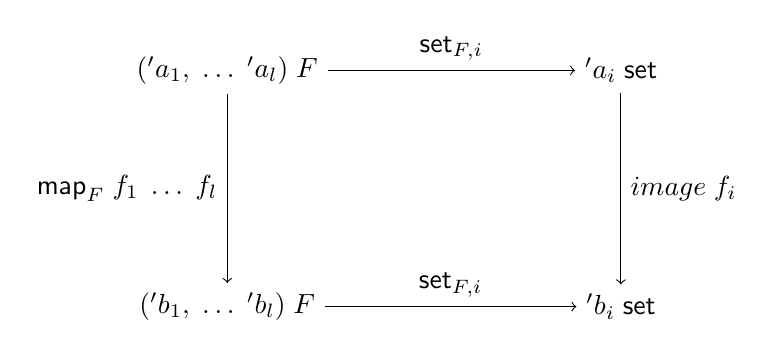
\begin{tikzpicture}[auto]
            % Nodes
            \node (aF) at (0,0) {\(('a_1,\; \dots\; 'a_l)\; F\)};
            \node (bF) at (0,-3) {\(('b_1,\; \dots\; 'b_l)\; F\)};
            \node (aset) at (5,0) {\('a_i\; \textsf{set}\)};
            \node (bset) at (5,-3) {\('b_i\; \textsf{set}\)};

            % Arrows
            \draw[->] (aF) to node[left] {\(\textsf{map}_F\; f_1\; \dots\; f_l\)} (bF);
            \draw[->] (aF) to node {\(\textsf{set}_{F,i}\)} (aset);
            \draw[->] (bF) to node{\(\textsf{set}_{F,i}\)} (bset);
            \draw[->] (aset) to node[right] {\(image\; f_i\)} (bset);
          \end{tikzpicture}
          \newline
          \footnotesize
          for all $i$ where $'a_i$ is a live variable of $F$
          \caption{$\textsf{set}_{F,i}$ as a natural transformation}
          \label{fig:set_nat}
        \end{figure}

        \noindent Another axiom of the setters and the mapper is the congruency \textsc{map\_cong} of the map function. It states that if two (lists of) functions $f_1 \dots f_l$ and $g_1 \dots g_l$ are equal when applied to the corresponding sets of all components of an $F$ (obtained through the setters), then mapping these two lists of functions over the $F$ each produces the same result. 

      \subsubsection{Bound and boundedness}
        Lastly, the \ac{BNF} needs a bound. This is an infinite cardinal that may depend on the cardinalities of the dead variables, but not on the of the live variables. The bound is used for the \textsc{set\_bd} axiom to ensure that the component sets obtained by the setters are bounded. This ensures that the branching of a recursively defined datatype is bounded.

      \subsubsection{Relator}
        The relator is used to build a relation on $F$ by relating the components of an $F$ element. It takes one relation for each live, that relates the corresponding type variables of the two $F$s that are to be related. As an example we give the type and definition of the relator as follows:
        \begin{align*}
          \textsf{rel}_\textsf{prod} ::\; &('a_1\; \Rightarrow\; 'a_2\; \Rightarrow\; \textsf{bool})\; \Rightarrow\; ('b_1\; \Rightarrow\; 'b_2\; \Rightarrow\; \textsf{bool})\Rightarrow\\
            &('a_1\; \times\; 'b_1)\; \Rightarrow\; ('a_2\; \times\; 'b_2)\; \Rightarrow\; \textsf{bool}\\
          \textsf{rel}_\textsf{prod}\; R\; S\; p_1\; p_2 :=\; & R\; (fst\; p_1)\; (fst\; p_2)\land S\; (snd\; p_1)\; (snd\; p_2)
        \end{align*}

        % extract the axioms from here?

    \subsection{BNF-axioms}
      A \ac{BNF} is characterized by map and set functions, a relator and a bound. We consider a \ac{BNF} $F$ with $l$ live variables and use the notation $\overline{f} = f_1 \dots f_l$. Furthermore, when we write $i$ as an index, we assume it to be in the range $1 \leq i \leq l$.
      We give the \ac{BNF}-axioms as follows:
      \begin{figure}
        \centering
        \begin{align}
          \textsc{map\_id: }& \textsf{map}_F\; \overline{id}\; x = x\\
          \textsc{map\_comp: }& \textsf{map}_F\; \overline{g}\; (\textsf{map}_F\; \overline{f}\; x) = \textsf{map}_F\; \overline{(g \circ f)}\; x\\
          \textsc{map\_cong: }& (\forall i.\; \forall z \in \textsf{set}_{F,i}\; x.\; f_i\; z = g_i\; z) \Longrightarrow 
            \textsf{map}_F\; \overline{f}\; x = \textsf{map}_F\; \overline{g}\; x\\
          \textsc{set\_map: }& \forall i.\; \textsf{set}_{F,i} (\textsf{map}_F\; \overline{f}\; x) = f_i\; \grave{\phantom{\_}}\; \textsf{set}_{F,i}\; x\\
          \textsc{bd: }& \textsf{infinite}\; \textsf{bd}_F \land 
            \textsf{regular}\; \textsf{bd}_F \land 
            \textsf{cardinal\_order}\; \textsf{bd}_F\\
          \textsc{set\_bd: }& \forall i.\; | \textsf{set}_{F,i}\; x | <_o \textsf{bd}_F\\
          \textsc{rel\_compp\_leq: }& \textsf{rel}_F\; \overline{R}\; \bullet\; \textsf{rel}_F\; \overline{Q}\; = 
            \textsf{rel}_F\; \overline{(R\; \bullet\; Q)}\\
          \textsc{in\_rel: }& \text{Weak Pullback Preservation WP}
        \end{align}
        \newline
        \footnotesize
        where $\grave{\phantom{\_}}$ is the image function on sets, $\bullet$ is the composition of relations and $<_o$ is the less than relation on cardinals
        \caption{The \ac{BNF} axioms}
        \label{fig:bnf_axioms}
      \end{figure}
      % Explain the other axioms

      While most of these properties are straightforward, we want to explain the preservation of weak pullbacks in more detail.
      \begin{equation}
        \textsf{rel}_F\; \overline{R}\; x\; y = 
          \exists z.\; (\forall i.\; \textsf{set}_{F,i}\; z \subseteq \{(a, b).\; R_i\; a\; b \}) \land 
          \textsf{map}_F\; \overline{fst}\; z = x \land \textsf{map}_F\; \overline{snd}\; z = y \label{eq:WP}
      \end{equation}
      The idea is that two elements $x$ and $y$ of the type $'a\; F$ are related through a relation $R$ iff there exists a $z$ that acts as a "zipped" version of $x$ and $y$. The components of this $z$ are $R_i$-related pairs of the components of $x$ and $y$, where the first position in the pair corresponds to $x$ and the second one to $y$.

    \subsection{Witnesses}
      
    \subsection{BNF examples}
      Further examples of \acp{BNF} are is the product type \type{($'a$, $'b$) prod}, a binary type constructor with infix notation \type{$'a\; \times\; 'b$}, and the type of finite sets \type{$'a$ fset}. The latter is interesting for the reason that it is a subtype of the set type, which is not a \ac{BNF}. By enforcing finiteness for the elements of the type it is possible to give a bound for the set function, fulfilling the \textsc{set\_bd} axiom, which is not possible for the unrestricted set type. Since unboundedness is the only reason that the set type is not a \ac{BNF}, \type{$'a$ fset} can be shown to be a \ac{BNF}.
      
      To show, how \acp{BNF} can be combined to create new ones, we consider the type constructor \type{($'a$, $'b$) plist} = \type{($'a\; \times\; 'b)$ list}. We define for it a map function ($\textsf{map}_\textsf{plist}$) and two set functions ($\textsf{set1}_\textsf{plist}$ and $\textsf{set2}_\textsf{plist}$) as well as a relator $\textsf{rel}_\textsf{plist}\; R\; S$. The exact definitions are given as such:
      \begin{align*}
        \textsf{map}_\textsf{plist}\; f\; g\; &= \textsf{map}_\textsf{list}\; (\textsf{map}_\textsf{prod}\; f\; g)\\
        \textsf{set1}_\textsf{plist}\; xs &= \textsf{set}_\textsf{list}\; (\textsf{map}_\textsf{list}\; fst\; xs)\\
        \textsf{set2}_\textsf{plist}\; xs &= \textsf{set}_\textsf{list}\; (\textsf{map}_\textsf{list}\; snd\; xs)\\
        \textsf{rel}_\textsf{plist}\; R\; S &= \textsf{rel}_\textsf{list} (\textsf{rel}_\textsf{prod}\; R\; S)
      \end{align*}
      \noindent where we use the standard map, set and relator functions of the list and product type.

      To show that \type{($'a$, $'b$) plist} is a \ac{BNF}, we have to prove the \ac{BNF}-axioms for it. Besides the definitions above, a bound $\textsf{bd}_\textsf{plist}$ is needed. We chose $natLeq$. 
      
      % TODO: EXPLAIN bd and natLeq

  \section{Subtype}
    We can carve out a subtype from a type constructor using the \textbf{typedef} command. 
    % The idea was to have this here to show that there exist BNFs that have a dead variable, that are not dead in an MRBNF (but bound). Maybe this idea has to go to the 3 chapter 

  \section{Map-Restricted Bounded Natural Functors (MRBNFs)}
    \acp{MRBNF} are a generalization of \acp{BNF}. Restricting the map function of a functor to \textit{small-support} functions or \textit{small-support bijections} for certain type variables allows us to reason about type constructors in terms of \ac{BNF} properties, even in cases where this would not be possible otherwise. We call type variables that that are restricted to small-support functions \textit{free} variables or \textit{frees} and those restricted to small-support bijections \textit{bound} variables or \textit{bounds}. This allows us to define \acp{MRBNF} with four types of variables (lives, frees, bounds and deads) as opposed to \acp{BNF} which only distinguish between lives and deads. 
    
    Consequently, for type constructors with variables that are considered dead in \ac{BNF} terms, we can declare some of them as free or bound variables, depending on the type. Consider for example the type of distinct lists \type{$'a$ dlist}, a subtype of \type{$'a$ list} that describes only lists containing pairwise distinct $'a$ elements. The issue with this type is that the standard map function on lists cannot guarantee that the resulting list is still distinct, i.e., that it is still part of the type. Thus in \ac{BNF} terms the type variable of \type{$'a$ dlist} is dead. However, by restricting the mapper to only use bijections, the distinctness of the resulting list can be ensured. Thus, it can be shown that \type{$'a$ dlist} is a \ac{MRBNF} with $'a$ as a bound variable.


    \acp{MRBNF} can be used in a \textbf{binder\_datatype} command to produce a datatype with bindings. 
    % binder_datatype command
    
    
  \begin{itemize}
    \item cite \cite{blanchette2019bindings}
  \end{itemize}

